% !TEX root = ../VPJ.tex

\chapter{Implementierung}
\label{sec:Implementierung}

Implementierung

\section{Programmstruktur}

\begin{figure}[htb]
    \centering
    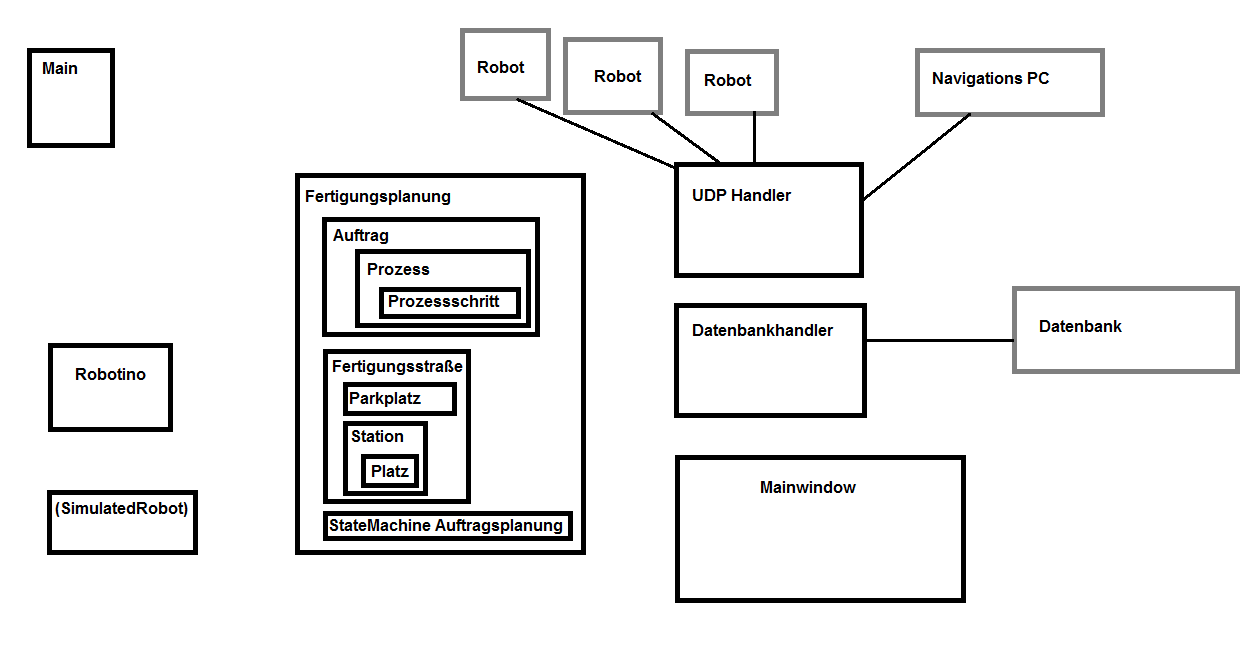
\includegraphics[width=0.9\textwidth]{Abbildungen/Klassendiagramm.PNG}
    \caption{Klassendiagramm}		
    \label{fig:Klassendiagramm}
\end{figure}



\section{Databasehandler}



\section{UDP-Handler} 
\label{sec:UdpHandler}



\section{Robotino} 

Die real existierenden Robotinos werden in der Klasse Robotino abgebildet. In der Klasse werden alle Daten gespeichert, die den Robotino beschreiben. Dazu gehören unter anderem die Position in x, y, der Winkel, eine eindeutige RoboterID. Weiterhin werden alle vom Robotino gesendeten Daten wie Status, Position, Error, Hindernis, Akku und Greifer gespeichert(vgl. \ref{sec:Gewerk2Protokoll}). 

Über ein isAlive-Tag kann validiert werden, dass der Robotino noch erreichbar ist. Das Defekt-Tag wird von Visualisierung und Auftragsplanung berücksichtigt, um den Robotino händisch außer Betrieb zu schalten. 

Es werden demnach deutlich mehr Daten über den Robotino gespeichert, als in der Datenbank hinterlegt werden. Dies kommt auch daher, dass über eine Änderung von manchen Werten ein Signal emittiert wird um über ein Event darauf zu reagieren. Diese Funktionalität ist über die Datenbank nicht gegeben. 

Beim Erzeugen einer Instanz eines Robotinos wird im Konstruktor sowohl die RoboterID festgeschrieben, als auch die IP-Adresse mit dem zugehörigen Sendeport und Empfangsport. Außerdem werden die Timer mit den zugehörigen Timeout-Funktionen verknüpft.

\subsection{Werte aktualisieren}

Wenn der zugehörige UDP-Handler eines Robotinos neue Werte bereitstellt (vgl. sec:UdpHandler) wird die Funktion UpdateValues() aufgerufen. Bei jedem Aufruf der Funktion wird der Robotino als Alive markiert und dies bei einer Änderung als Signal emittiert. Zusätzlich wird der 30 Sekunden laufende AliveTimer gestartet oder zurückgesetzt. 

Wenn sich der anliegende Robotererror geändert hat wird dieser kategorisiert und den bekannten Robotererrortypen (vgl. \ref{sec:Gewerk2Protokoll}) zugeordnet. Folgend wird ein Signal emittiert, welches eine Änderung des Errors anzeigt und den Errortyp beinhaltet.

Bei einer Änderung von Greifer, Akku, Hindernis oder UDPAlive wird jeweils der Wert gespeichert und die Änderung über ein spezifisches Signal emittiert. 

Eine Statusänderung des Robotinos bewirkt eine Vorauswertung des empfangenen Statuswerts. Der zusammengesetzte Status wird wieder in seine drei Bestandteile zerlegt und über ein Signal bekanntgemacht. Bei einem Status von über 200 wird die Roboterposition ebenfalls gespeichert. 

\subsection{Visualisierungsfunktionen}

Bei Empfangen von Navigationsdaten vom Navigationsrechner zu einem Robotino wird in der Funktion UpdatePosition() die Roboterposition angepasst. Dazu wird zunächst überprüft, ob sich die Position um mehr als 2 in X- und Y-Richtung und um mehr als 1 im Winkel geändert hat. Damit wird eine Glättung der Roboterposition erzeugt und ein "`zittern"' in der Visualisierung aufgrund der schwankenden Position unterdrückt. 

Der Sonderfall, dass alle drei empfangenen Werte 0 sind bedeutet, dass der Navigationsrechner den Robotino verloren hat. In diesem Fall wird die Roboterposition nicht aktualisiert und statdessen ein NavigationsTimer gestartet. Wenn nach fünf Sekunden keine neue Robotinoposition erkannt wird, so wird der Robotino in der Visualisierung verdeckt. Dadurch wird eine kurzzeitige Verdeckung durch z.B. die Kabelgänge an den Stationen der Robotino immer noch angezeigt und verschwindet nicht.

Sobald sich der Alive-Tag ändert wird in der Visualisierung die RoboterAlive-LED angepasst. Ein Roboter wird als Alive gewertet bei Aufruf der Funktion UpdateValues(). Wenn der AliveTimer abläuft wird der Robotino als nicht Alive gewertet. Das führt dazu, dass ein Robotino auch als lebend angezeigt wird, wenn die Kommunikation nicht vollständig funktioniert, solange dieser seinen Status an den Fertigungsplanungsrechner sendet. Nach maximal 30 Sekunden wird ein Absturz der Kommunikation erkannt und der Robotino wird ncht länger in der Auftragsvergabe berücksichtigt. 

\section{Auftrag, Prozess, Prozessschritt} 
\label{sec:AuftragProzessSchritt}

Die im Programm auftretenden Aufträge sind in einer bestimmten Struktur organisiert. Diese variiert zu der in der Datenbank abgespeicherten Struktur. So wird über die Visualisierung ein Auftrag angelegt. Jeder so angelegte Auftrag beinhaltet ein oder mehrere Prozesse. In der Datenbank sind dies komplementär gesehen die Werkstücke. Jeder Prozess besteht aus mehreren Prozessschritten, die den genauen Ablauf eines Prozesses beschreiben. 

Auftrag, Prozess und Prozessschritt sind in verschiedene Klassen geschrieben. Folgend werden diese Klassen näher beleuchtet. 

\subsection{Prozessschritt}
\label{sec:Prozessschritt}

Ein Prozessschritt besteht aus genau einer Stations-ID verknüpft mit einer festen Bearbeitungsdauer in Sekunden. Dies beschreibt für einen Teil eines Prozesses. In einer Fortschritts-Flag wird festgehalten, ob der Prozessschritt bereits bearbeitet wurde, oder noch bearbeitet werden muss. 

Der Prozessfortschritt kann ein Signal emittieren, welches anzeigt, dass sich der Fortschritt geändert hat.

\subsection{Prozess}
\label{sec:Prozess}

Ein Prozess, in der Datenbank Werkstück, beinhaltet eine Liste von Prozessschritten. Diese Liste bestimmt mit ihrer Reihenfolge und Länge die Bearbeitungsvorschrift für ein Werkstück. Jeder Prozess besitzt zudem einen Fortschritt, eine eindeutige ID und eine ReferenzID. 

Mit der eindeutigen ID kann später ein Prozess innerhalb des Programms wiedergefunden werden. Nur die in Aufträgen befindlichen Prozesse erhalten eine aufsteigende laufende Nummer als eindeutige ID. Die in der Initialisierung erzeugten Prozesse oder die über die Visualisierung erzeugten Prozesse (folgend Referenzprozesse) erhalten keine spezielle eindeutige ID, sondern eine aufsteigende eindeutige ReferenzID. Dies führt dazu, nicht alle Informationen in den einzelnen Prozessen halten zu müssen, sondern auf den initialisierten Referenzprozess zugreifen zu können. 

Die ReferenzID eines Prozesses einhält die eindeutige ID des zugehörigen Referenzprozesses. 

Zur Prozesskontrolle gibt es zusätzlich noch verschiedene Flags die den Status des Prozesses widerspiegeln. Dazu gehört ein Blocked- und ein InProgress-Flag. Das InProgress-Flag wird gesetzt, sobald ein Werkstück an einer Station bearbeitet wird. Das Blocked-Flag kann über die Hard-Code Area (vgl. Kapitel \ref{sec:HardCode}) gesetzt werden und verhindert eine weitere Bearbeitung. 

Jeder Prozess enthält einen Timer, der die verbrauchte Zeit an einem Arbeitsplatz kontrolliert. Der Timer wird gestartet, sobald ein Werkstück an einer Station bearbeitet wird, die nötige Zeit wird dem zugehörigen Prozessschritt entnommen. Bei Ablauf des Timers wird die Funktion TimerElapsed() aufgerufen, in der der zugehörige Prozessschrittfortschritt auf fertig gesetzt und das InProgress-Flag zurückgesetzt wird. 

Über die beiden Signale ProzessFinished und FortschrittUpdated kann bekannt gemacht werden, dass sich ein Fortschritt eines Prozesses geändert hat oder die Arbeit an einer Station beendet wurde und das Werkstück bereit ist für Abholung.

Mit der im Prozess enthaltenen Funktion UpdateFortschritt() wird der Fortschritt eines Prozesses anhand der beinhalteten Prozessschritte aktualisiert. Dazu wird die Prozessschrittliste durchgegangen und für jeden Prozessschritt, der als fertig markiert wurde ein entsprechender Fortschritt zum Prozessfortschritt addiert. Die einzelnen Prozessschritte sind dabei so gewichtet, dass die Summe aus allen Prozessschritten, wenn alle abgeschlossen sind, 100 ergibt. Durch Rundungsfehler können in der aktuellen Umsetzung nicht mehr als 25 Prozessschritte je Prozess sauber dargestellt werden. Sollten mehr Prozessschritte erforderlich sein, so müsste die Fortschrittsberechnung angepasst werden.

\begin{figure}[htb]
    \centering
    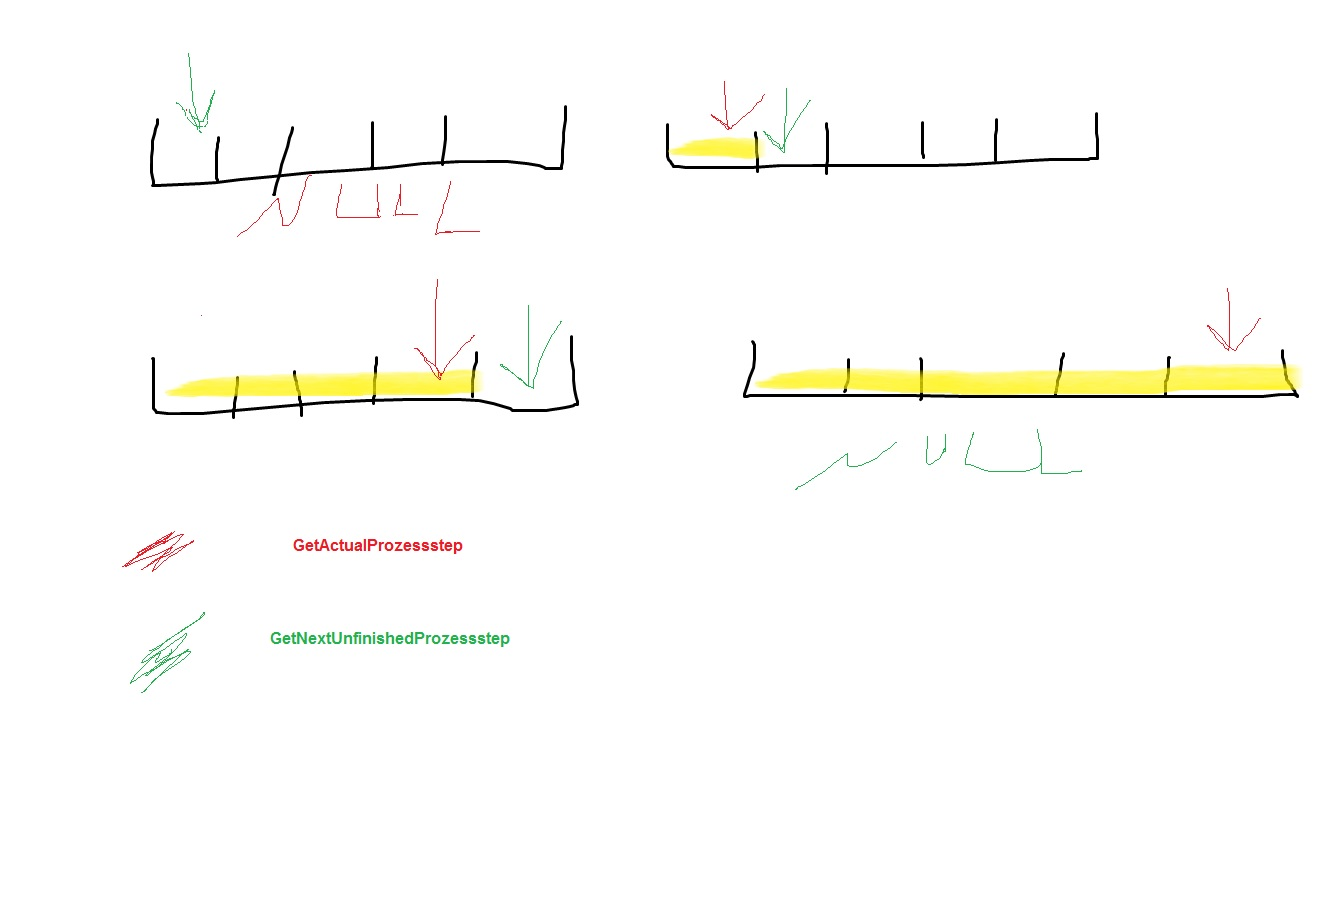
\includegraphics[width=0.9\textwidth]{Abbildungen/GetProzessstep.PNG}
    \caption{Visualisierung des Rückgabewertes der Funktionen GetNextUnfinishedProzessstep() und GetActualProzessstep()}		
    \label{fig:GetProzessstepFunktionen}
\end{figure}

Um auf den richtigen Prozessschritt innerhalb der Liste zuzugreifen sind zwei unterschiedliche Funktionen implementiert. Beide Funktionen unterscheiden sich ausschließlich in ihrem Rückgabewert. In Abbildung \ref{fig:GetProzessstepFunktionen} sind alle möglichen Fälle Prozessschrittliste leer oben links, ein oder mehrere Prozessschritte in der Liste oben rechts und unten links und Liste voll unten rechts dargestellt. Dabei ist zu erkennen, dass die Funktion GetNextUnfinishedProzessstep() immer den nächsten Prozessschritt zurückliefert, der noch nicht bearbeitet wurde. Bei voller Liste wird NULL zurückgegeben. Anders hierzu die Funktion GetActualProzessstep(), die NULL bei leerer Liste zurückgibt und sonst den letzten fertigen Prozessschritt. 

Die Funktion GetActualProzessstep() wird in der Fertigungsplanung zur Planung der Aufträge verwendet (siehe \ref{sec:CheckAuftrag}). GetNextUnfinishedProzessstep() findet Anwendung sobald auf einem aktuellen Prozess eine Änderung auftritt oder umgesetzt werden soll. Wenn beispielsweise der Timer abgelaufen ist, wird in der Funktion TimerElapsed() über der zurückgegebene Prozessschritt als fertig markiert.

\subsection{Auftrag}
\label{sec:Auftrag}

Die Klasse Auftrag enthält eine Liste von Prozessen und darin enthaltenen Prozessschritten und bündelt somit alle drei Klassen. Ähnlich dem Prozess gibt es einen Fortschritt, der sich anteilig aus den einzelnen Prozessfortschritten errechnet und eine eindeutige ID mit derer der Auftrag wiedergefunden und verwaltet werden kann. 

Mit dem Signal FortschrittUpdated kann bekannt gemacht werden, dass sich der Fortschritt geändert hat und z.B. die Visualisierung aktualisiert werden. Das Signal wird gesendet, sobald die Funktion UpdateFortschritt() aufgerufen wurde. In dieser Funktion werden alle enthaltenen Prozesse auf ihren Fortschritt überprüft und im Auftrag gegebenenfalls angepasst. Die Fertigungsplanung verknüpft Auftrag, Prozess und Prozessschritt derartig, dass ein Fortschrittsupdate innerhalb eines Prozessschrittes eine Aktualisierung des Prozessfortschritt hervorruft. Dies wiederum lässt den entsprechenden Auftragsfortschritt aktualisieren (siehe Listing \ref{lst:Auftragserzeugung}).

Ein bestimmter Prozess aus der Liste kann über die Funktion GetProzessByID() mit seiner eindeutige ID zurückgegeben werden. 

Weiterhin werden zwei Funktionen bereitgestellt, die von der Fertigungsplanung genutzt werden um Prozesse oder Prozessschritte zu erhalten. Die Funktion GetNextUnfinishedProzesssteps() gibt, mit Hilfe der Funktion GetNextUnfinishedProzessstep() aus dem Prozess, eine Liste aller entsprechenden Prozessschritte zurück (vgl. Abschnitt \ref{sec:Prozess}). Über die Funktion GetAllUnfinishedProzesses() werden alle Prozesse zurückgegeben, die noch unfertige Prozessschritte enthalten, sofern diese nicht blockiert sind. Hiermit werden in der Fertigungsplanung die zu bearbeitenden Prozesse ausgewählt (siehe \ref{sec:CheckAuftrag}).

\section{Fertigungsplanung}
\label{sec:Fertigungsplanung}

Die Klasse Fertigungsplanung enthält alle verfügbaren Roboter, die Datenbankschnittstelle, die abzuarbeitenden Aufträge (vgl. Abschnitt \ref{sec:AuftragProzessSchritt}), die Fertigungsstraße und eine State Machine zur Verteilung von Roboteraufträgen. Außerdem wird auf Events reagiert, die von der Visualisierung oder anderen Quellen kommen. Zu den Events gehören Statusänderungen des Roboters, hinzufügen von Aufträgen oder Prozessen und Funktionen, die über die Hard-Code Area (vgl. Kapitel \ref{sec:HardCode}) angestoßen werden können. 
In der Fertigungsplanungsklasse werden somit alle Funktionalitäten gebündelt, die nicht direkt mit der Visualisierung zusammenhängen. 

\subsection{Initialisierung}
\label{sec:Fertigunginit}

Um die Fertigungsplanung zu initialisieren wird zunächst in der Funktion InitProzesses() ein Grundzustand hergestellt, in der mindestens 5 Prozesse vorhanden sind. Dazu werden zunächst über einen Datenbankaufruf alle dort verfügbaren Prozesse in eine Liste geschrieben. 

Sollte die Liste weniger als 5 Elemente beinhalten, also in der Datenbank zu Programmstart weniger als 5 Prozesse vorhanden sein, so werden 5 neue zuvor definierte Prozesse (Abschnitt \ref{sec:Standardprozesse}) angelegt und die Liste so überschrieben. 

Die erzeugten Prozesse werden abschließend in die Datenbank geschrieben. Außerdem erhalten alle Prozesse gemäß ihrer Schritte und Dauer in der Visualisierung einen entsprechenden Tooltip (vgl. Kapitel \ref{sec:tooltips}). 

Die Prozessliste kann über die Funktion AddProzess() dynamisch während das Programm läuft erweitert werden. Dies geschieht bei absenden eines eingestelltes Prozesses in der Visualisierung (\ref{sec:Prozesseingabe}). 

\subsubsection{Aufträge hinzufügen}

Durch Einstellen und Absenden eines Auftrags in der Visualisierung (\ref{sec:Auftragseingabe}) wird die Funktion AddAuftrag() aufgerufen. In dieser Funktion wird zunächst ein leeres Auftragsobjekt erzeugt und diesem die nächst höhere Auftragsnummer aus der Datenbank zugeordnet.  

Für jeden Prozesseintrag aus der Visualisierung wird nun die angegebene Anzahl des jeweiligen Prozesses eine Prozesskopie erzeugt. Den so kopierten Prozessen werden alle zugehörigen Prozessschritte als Kopie angehängt, um eigenständige Aufträge zu erhalten. Zuletzt werden die Prozesse und Aufträge miteinander verknüpft (siehe Listing \ref{lst:Auftragserzeugung}).

\begin{lstlisting}[frame=single, breaklines=true, numbers=left, stepnumber=2, firstnumber=1, numberstyle = \tiny, caption=Auftragserzeugung und Verknüpfungen,label=lst:Auftragserzeugung]
Auftrag *A = new Auftrag();

for (int prozesscounter = 0; prozesscounter < 5; prozesscounter++) //5 Prozess UI Elemente
{
    for (int i = 0; i < Avalues[prozesscounter]; i++) //Anzahl der eingegebenen Prozesszahl
    {
        Prozess *p = new Prozess();
        [...]  // Prozess + Prozessschritte kopieren
        A->Prozesse.append(p);
        QObject::connect(p, &Prozess::FortschrittUpdated, A, &Auftrag::UpdateFortschritt);
        QObject::connect(p, &Prozess::ProzessFinished, this, &Fertigungsplanung::StationReady);
    }
}
\end{lstlisting}

Abschließend wird der Auftrag der Auftragsliste angehängt, an die Datenbank gesendet und ein Auftragsitem in der Visualisierung erzeugt (Kapitel \ref{sec:Auftragsuebersicht}). 

\subsubsection{Standardprozesse}
\label{sec:Standardprozesse}

Folgend werden die in Abschnitt \ref{sec:Fertigunginit} erwähnten Standardprozesse näher beleuchtet. 

Um ein möglichst ausgeglichenes Fertigungsbild zu schaffen wurden die fünf Standardprozesse so untereinander abgestimmt, dass diese unterschiedlichen Kriterien genügen. 

Zunächst wurde darauf geachtet, dass die Prozesse unterschiedlich viele Prozessschritte beinhalten. Abbildung \ref{fig:Fahrweganalyse} kann entnommen werden, dass die Prozesse zwischen zwei und sechs einzelne Prozessschritte erfordern. In der Abbildung ist weiterhin dargestellt, welche Station als Start und Ziel je Prozessschritt angefahren wird. 

\begin{figure}[htb]
    \centering
    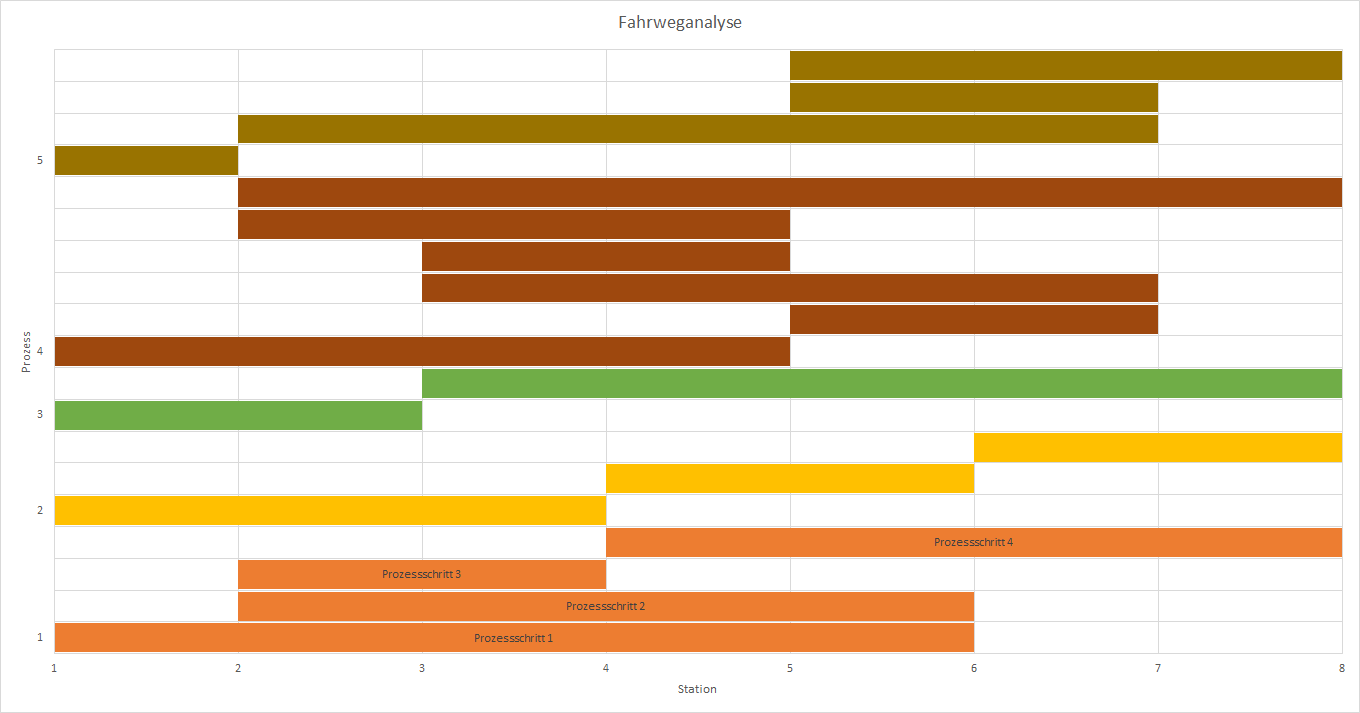
\includegraphics[width=0.9\textwidth]{Abbildungen/Fahrweganalyse.PNG}
    \caption{Diagramm Fahrweganalyse}		
    \label{fig:Fahrweganalyse}
\end{figure}

Zu erkennen ist, dass jeder Prozess bei Station 1 beginnt und in Station 8 endet. Die Einzelnen Prozesse (siehe farbliche Unterscheidung) sind dabei von unten nach oben zu lesen, beginnend mit Prozessschritt 1. 

Aus dem Diagramm können weiterhin potentielle Kollisionsherde und "`Staugefahren"' erkannt werden. Die Standardprozesse wurde so angepasst, dass alle Stationen möglichst gleichmäßig häufig durchfahren werden. Weiterhin kann aus dem Diagramm abgelesen werden, ob durch ungünstige Auftragsplanung ein Deadlock angefahren werden kann, also alle Aufträge irgendwann durch andere Aufträge blockiert sein können. Da keine Schleifen zwischen den Stationen entstanden sind kann gewährleistet werden, dass alle Aufträge in jeder Belegung nach einiger Zeit abgearbeitet werden können, wenn die Werkstücke in Station 8 entnommen werden.

Das Diagramm in Abbildung \ref{fig:Stationsanalyse} zeigt eine genauere Analyse der Stationen. Angenommen wird, dass jeder der Standardprozesse genau ein mal abgearbeitet wird. Auf der linken y-Achse, die zu den bunten Säulen gehört, ist die Belegungsdauer jeder Station in Sekunden angegeben. Die rechte, den hellgelben Säulen zugeordnete y-Achse bezeichnet die Anzahl der Anfahrten an eine Station. 

\begin{figure}[htb]
    \centering
    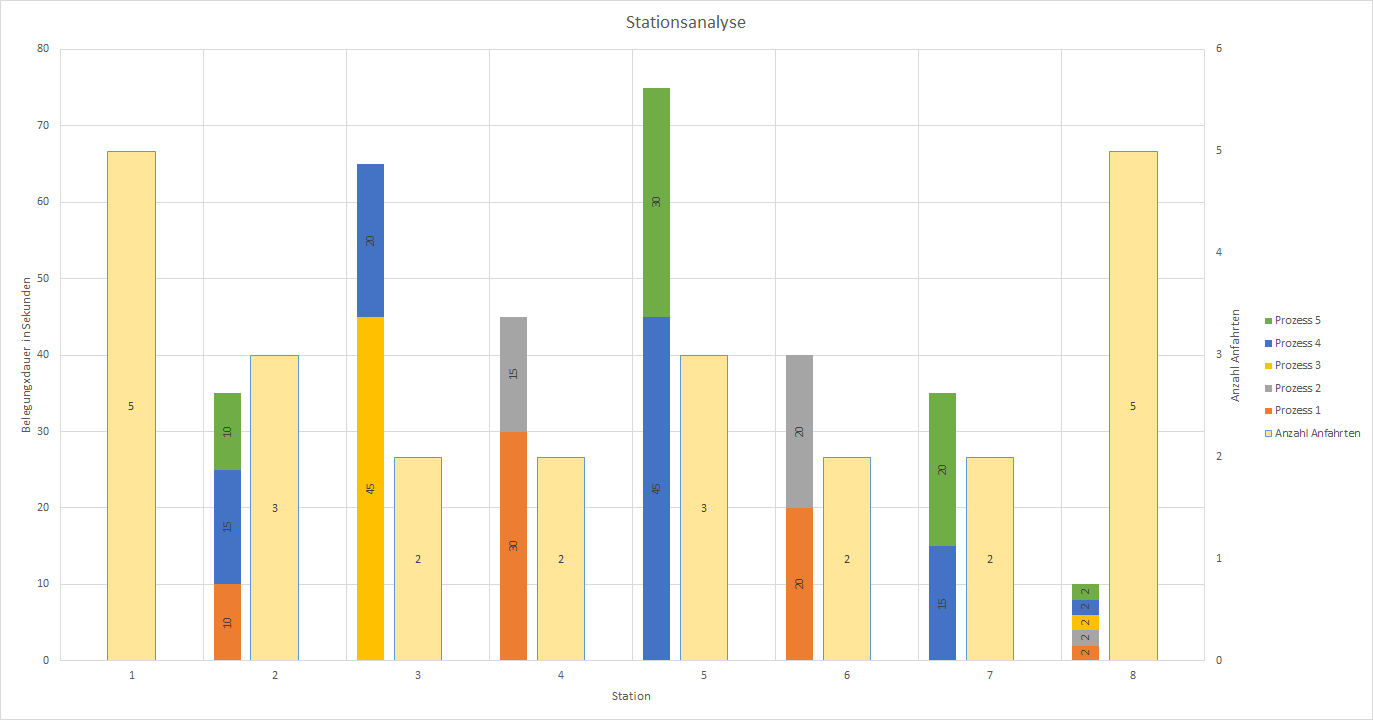
\includegraphics[width=0.9\textwidth]{Abbildungen/Stationsanalyse.PNG}
    \caption{Diagramm Stationsanalyse}		
    \label{fig:Stationsanalyse}
\end{figure}

Es ist zu erkennen, dass Station 1 und 8 genau fünf mal angefahren werden, also je Prozess ein mal. Die weiteren Stationen 2 bis 7 werden zwei- bis dreimal angefahren. So wird sichergestellt, dass die Stationen möglichst gleichmäßig belastet werden. 

Die farblich unterschiedlichen Säulen zeigen die kürzeste Belegungsdauer der Arbeitsplätze an. Die Balken ergeben sich durch die Dauer eines einzelnen Prozessschrittes an einem Arbeitsplatz. Es  Belegungsdauer für alle Prozesse zwischen 35 und 75 Sekunden je Station liegt. Die 2 Sekunden Bearbeitungsdauer je Prozess an Station 8 sind dabei vernachlässigt worden und gewährleisten nur ein sicheres Herausnehmen der Werkstücke durch den Menschen, ohne dass sich der Roboter noch im Entladezyklus befindet. 

Als Besonderheit ist an Station 5 zu erkennen, dass es drei Anfahrten, aber nur zwei verschiedene Prozesse gibt. Dies liegt darin begründet, dass Prozess 4 Station 5 zwei mal anfährt mit verschieden langen Zeiten. Dadurch ist die Gesamtzeit in Station 5 auch am höchsten, gehört jedoch zu großen Anteilen zum selben Prozess. Station 2 hat die kürzesten Bearbeitungszeiten je Prozess, da diese Station von drei verschiedenen Prozessen angefahren wird. Gegensätzlich dazu ist die Bearbeitungszeit an Station 23 von Prozess 3 mit 45 Sekunden sehr hoch angesetzt, da dieser Prozess keine weitere Station anfährt. 

Es wurde versucht, die durchschnittliche Belegungsdauer der Stationen anzugleichen, um alle Arbeitsplätze möglichst homogen auszulasten. Zu erkennen ist, dass die minimale

Als Nebeneffekt ergibt sich, dass die Roboter möglichst ausgeglichen über die gesamte Fertigungsstraße fahren und die Gefahr von Staus oder Kollisionen dadurch verringert wird. 

\subsection{Roboter Statusänderungen}

Wenn eine der in der Fertigungsplanung enthalten Roboterklassen ein Event feuert, welches eine Statusänderung beinhaltet (vgl. Kapitel \ref{sec:UdpHandler}), wird über Funktionen in der Fertigungsplanung auf diese reagiert. So wird der Greifer oder das Statusflag eines Roboters bei einer Änderung aktualisiert. Beim Empfanges eines Errorevents des Roboter wird je nach Errortyp eine Meldung ausgegeben und individuell auf die Robotererror reagiert. 

Weiterhin wird durch Ablauf des Timers eines Arbeitsplatzes dieser in der Fertigungsstraße aktualisiert und auf bereit geschaltet. 


\subsubsection{Roboterstatus geändert}

Bei Änderung des Roboterstatus wird die Funktion OnRobotStatusChanged() aufgerufen. Dabei wird zunächst der aufrufende Roboter ausgewählt und zwischengespeichert. Sollte sich der Status des Roboter auf eins geändert haben, also der Roboter auf dem Weg zu etwas ist, so wird unterschieden ob sich der Roboter auf einem Parkplatz oder einem Arbeitsplatz befunden hat.

Von einem Parkplatz (auch Ladestation) kommend wird dieser in der Datenbank und der Visualisierung wieder freigegeben. Wenn der Roboter zuletzt an einer Station war, so wird diese jetzt für andere Roboter freigegeben und der Roboter wird in der Datenbank aus dem Arbeitsplatz gelöscht. 

\subsubsection{Greiferstatus geändert}

Die Prozessaktualisierungen basieren auf der Änderung des Greifers des Roboters. Es wird vorausgesetzt, dass sich der Greifer zu keinem Zeitpunkt willkürlich öffnet oder schließt, sondern nur bei Aufnahme oder Abgabe eines Werkstücks an einer Station. 

Das Schließen des Greifers eines Roboters bedeutet somit immer, dass ein Werkstück aufgenommen wurde. Somit wird in der Datenbank der Arbeitsplatz, an dem sich der Roboter befindet freigegeben und kann für andere Aufträge genutzt werden. Der Arbeitsplatz wird in der Visualisierung und der Datenbank freigegeben. Zuletzt wird der Tooltip des Arbeitsplatzes (vgl. Kapitel \ref{sec:tooltips}) auf einen leeren String gesetzt. 

Beim Öffnen des Greifers wird ein Werkstück in einen Arbeitsplatz einer Station gelegt. Daraufhin wird die Zuordnung des Werkstücks zu dem entsprechenden Roboter gelöscht. Mit der Werkstücks-ID kann nun aus der Auftragsliste der zugehörige Prozess identifiziert werden. Der Timer des so gefundenen Prozesses wird jetzt gestartet, somit läuft die Bearbeitung des Werkstücks an dem Arbeitsplatz. In der Visualisierung und Datenbank wird der Arbeitsplatz von reserviert auf belegt aktualisiert.

Weiterhin wird das Werkstück, dass dem Roboter zu diesem Zeitpunkt zugeordnet ist an der Station an der sich der Roboter zuletzt aufgehalten hat gelöscht und der zugehörige Arbeitsplatz wird freigegeben. 

\subsubsection{Roboter Error geändert}

Bei Auftreten eines Errors im Roboter wird je nach Typ eine Error-Meldung ins Log geschrieben. 

Die Error-Meldungen des Roboters wurden bewusst nicht automatisiert behandelt, da dem Benutzer die Kontrolle über das Gesamtsystem behalten sollte. Somit muss je nach Fehlertyp eine unterschiedlicher Lösungsweg verfolgt werden. 

Die auftretenden Fehler und der Lösungsweg ist in Kapitel \ref{sec:Error} zu finden. 

\subsection{Hard-Code Funktionen}

Die mit der Hard-Code Area erzeugten Befehle aus der Visualisierung (vgl. Kapitel \ref{sec:HardCode}) werden in verschiedenen Funktionen verarbeitet. So wird beispielsweise der Parkplatz oder eine Station in Datenbank und Visualisierung freigegeben, ein Roboter defekt geschaltet oder ein Arbeitsplatz als defekt markiert oder repariert. 

\subsection{Zustandsdiagramm}

Das Zustandsdiagramm in Abbildung \ref{fig:Auftragsplanung} beschreibt die Logik der Auftragsvergabe an die Roboter. Das Diagramm wurde anschließend als State Machine (vgl. \ref{sec:StateMachines}) implementiert. 

\begin{figure}[htb]
    \centering
    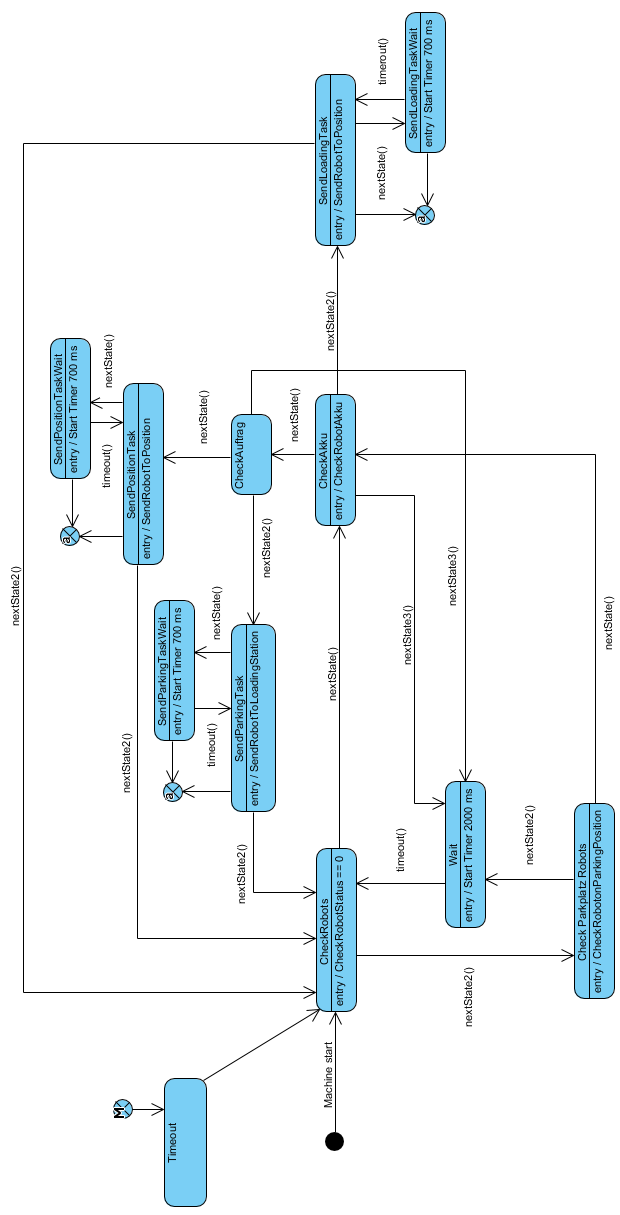
\includegraphics[width=0.8\textwidth]{Abbildungen/Auftragsplanung_rotated.PNG}
    \caption{Zustandsdiagramm der Auftragsplanung}		
    \label{fig:Auftragsplanung}
\end{figure}

In der Abbildung sind die Zustände mit Namen dargestellt. Alle Zustände haben eine komplementäre Funktion, die nach einem Zustandswechsel als Entry-Action aufgerufen wird. Eine genaue Funktionsbeschreibung der Zustände ist in Kapitel \ref{sec:StateMachineImplementierung} zu finden. Um zwischen den Zuständen zu wechseln werden die mit Pfeilen eingezeichneten Transitionen verwendet. Die Pfeilbeschriftung beinhaltet dabei das Signal, welches für den Zustandswechsel genutzt wird. Um das Diagramm übersichtlich zu gestalten, wurden die Timeout-Transitionen nicht vollständig eingezeichnet, sondern enden in einem kreisförmigen Xa-Zustand. Dieser führt direkt zu dem XM-Zustand oben links und leitet in den Zustand Timeout weiter. 

\subsection{State Machine Implementierung}
\label{sec:StateMachineImplementierung}

Im Quellcode werden zunächst alle Zustände erzeugt und der State Machine hinzugefügt. Anschließend werden alle Transitionen zwischen den Zuständen erzeugt und der State Machine hinzugefügt. Hierbei werden definierte Signale genutzt, die zuvor in der Header Datei deklariert wurden. In der Main-Funktion werden abschließend die Zustände mit den entsprechenden zugehörigen Funktionen verknüpft (vgl. \ref{sec:Main}). 

Um die State Machine zu starten wird, nachdem der Initialzustand bekannt gemacht wurde, die Start-Funktion aufgerufen. Eine verkürzte Darstellung der Aufrufe ist in Listing \ref{lst:StartStateMachine} abgebildet. 

\begin{lstlisting}[frame=single, breaklines=true, numbers=left, stepnumber=2, firstnumber=1, numberstyle = \tiny, caption=Start und Initialisierung der State Machine,label=lst:StartStateMachine]
    QStateMachine StateMachine;
    QState *StateCheckRobots = new QState;

    StateMachine.addState(StateCheckRobots);
    StateCheckRobots->addTransition(this, SIGNAL(nextState()), StateCheckAkku);

    StateMachine.setInitialState(StateCheckRobots);
    StateMachine.start();

    QObject::connect(StateCheckRobots, &QState::entered, this, &Fertigungsplanung::CheckRobots);
\end{lstlisting}

\subsubsection{Zustand CheckRobots}

Im Initialzustand der State Machine, CheckRobots, werden alle vier Roboter nacheinander auf Bereitschaft überprüft. Die Reihenfolge der zu überprüfenden Roboter wird dabei durch einen hierfür entwickelten Shuffle-Algorithmus (\ref{sec:shuffle}) bestimmt. 

Ein Roboter gilt als bereit, wenn er als Status 0 zurückgibt, nicht als defekt markiert ist und als lebend gilt. Sobald ein geprüfter Roboter alle drei Kriterien erfüllt wird dieser ausgewählt und in den weiteren Zuständen, gefolgt von CheckAkku, genutzt. Die anderen Roboter werden bis zum nächsten Aufruf des Zustands CheckRobots vernachlässigt.

Sollte keiner der vier Roboter alle drei Kriterien erfüllen wird in den Zustand CheckParkplatzRobots gewechselt.

\subsubsection{Zustand CheckParkplatzRobots}

Wie im Zustand CheckRobots werden alle vier Roboter anhand von Kriterien auf Bereitschaft überprüft. Dazu wird ebenfalls die Reihenfolge zufällig bestimmt.

Anstatt den Roboterstatus wie beim Zustand CheckRobots auf 0 zu prüfen, wird ein Status zwischen 201 und 204 erwartet. Diese vier Stati repräsentieren die vier Parkplätze auf denen sich ein Roboter befinden kann. 

Durch die Aufteilung der Zustände CheckRobots und CheckParkplatzRobots erfolgt eine Priorisierung der Roboter, die sich bereits in den Stationen befinden und einen Auftrag fertig abgearbeitet haben. Nur wenn kein Roboter in den Stationen verfügbar ist wird auf die auf den Parkplatz befindlichen Roboter zurückgegriffen. Dadurch werden Situationen vermindert, in denen sich die Roboter bei der Stationsarbeit gegenseitig behindern.

Sollte keiner der auf den Parkplatz befindlichen Roboter alle weiteren Kriterien erfüllen wird in den Zustand Wait gewechselt.

\subsubsection{Zustand Wait}

Da in Qt aufgrund der eventbasierten Programmierung (vgl. \ref{sec:Eventbasiert}) keine Endlosschleifen vorgesehen sind wurde im Zustand "`Wait"' mittels Timer die Zustandsmaschine künstlich verlangsamt. Ein Entfernen des Zustands führt zum Programmabsturz, da in kürzester Zeit die interne Eventliste voll geschrieben wird. Auf externe Events wie Mauseingaben oder Ereignisse vom Betriebssystem könnte somit nicht mehr reagiert werden. 

Durch den Zustand Wait können andere Programmevents und Ereignisse des Betriebssystems abgearbeitet werden, während 2000 ms auf das timeout()-Signal des Timers gewartet wird. 

Nach Ablauf des Timers wird in den Initialzustand CheckRobots gewechselt.

\subsubsection{Zustand CheckAkku}

Der Zustand CheckAkku gewährleistet einen Tiefentenladungsschutz der Roboter. Sobald ein Roboter in den ersten beiden Zuständen ausgewählt wurde wird überprüft, ob sein Akkustand größer gleich 25 Prozent ist. Es wird davon ausgegangen, dass kein Auftrag plus eine Fahrt zum Laden mehr als 25 Prozent Akku verbraucht. Der Wert wurde empirisch ermittelt. 

Sollte der Akkustand unter 25 Prozent liegen, wird der Roboter über Zustand SendLoadingTask zu einer freien Ladestation geschickt. Wenn keine Ladestation frei ist wird in den Zustand Wait gewechselt. 
Bei einem Akkustand von über 25 Prozent wird der Zustand CheckAuftrag aufgerufen. 

\subsubsection{Zustände SendLoadingTask, SendParkingTask, SendPositionTask}

Um bei Kommunikation mit den Robotern in den Zuständen SendLoadingTask, SendPositionTask und SendParkingTask sicherzustellen, dass die Nachricht empfangen wurde, wird diese mehrfach gesendet, bis die Übertragung erfolgreich war (siehe Kapitel \ref{sec:sequenzdiagram}). Es wird nach jedem Sendevorgang ein kurzer Wartezustand aufgerufen, der, gleich dem Zustand Wait, einen Programmabsturz verhindert. Mit dem individuellen Wartezustand kann ebenfalls das bei aktuell 700 ms angesetzte Sendeintervall eingestellt werden. 

Aus allen den drei Send......Task Zuständen und ihren zugehörigen Wartezuständen kann über ein Ablauf eines Timers in den Zustand Timeout gewechselt werden. Der Timer wird beim erstmaligen Eintritt in einen der Zustände Send......Task gestartet und läuft nach 25 Sekunden ab. Dieser Timer gewährt eine Absturzsicherheit des Programms bei Roboterausfall oder anderweitigem Fehlschlagen der Kommunikation. 

In allen drei Send.....Task Zuständen wird ein erfolgreicher Sendevorgang damit erkannt, dass der Roboterstatus nicht mehr 0 ist, und der Roboter sich nicht mehr auf einem Parkplatz befindet. Solange die beiden Bedingungen nicht erfüllt sind wird weiter an den Roboter gesendet. 

Wenn im Zustand SendLoadingTask die Nachricht erfolgreich versendet wurde, wird der Timer für das Timeout gestoppt, und die benötigte Ladestation in der Visualisierung und in der Datenbank reserviert. Abschließend wird in den Initialzustand gewechselt.

Der Zustand SendParkingTask verhält sich Analog dem SendLoadingTask, nur wird bei erfolgreicher Nachrichtenversendung der benötigte Parkplatz reserviert.

Bei dem Zustand SendPositionTask, in dem ein Auftrag aus der Planung an den Roboter verschickt wurde, werden nach erfolgreichem Nachrichtenversand mehrere Aktionen durchgeführt. Zunächst wird der Timeout-Timer gestoppt. Sollte der Auftrag den ersten Prozessschritt, also das Abholen eines Werkstücks im Lager an Station 1, beinhalten wird der Schreibkopf des RFID neu beschrieben. In der Datenbank wird außerdem dem Start- und Zielarbeitsplatz der genutzte Roboter zugeordnet. Am Startarbeitsplatz wird das vorhandene Werkstück in der Datenbank entfernt und dem Zielarbeitsplatz zugeordnet. Die beiden Stationen werden außerdem Reserviert um zu verhindern, dass ein anderer Roboter an die zu bearbeitenden Stationen geschickt wird. Somit ist eine erste Kollisionsvermeidung implementiert. Zuletzt wird in der Datenbank das genutzte Werkstück dem Roboter zugewiesen. Auch in der Visualisierung werden Start- und Zielarbeitsplatz reserviert. Schlussendlich wird in der Visualisierung der Tooltip (vgl. Kapitel \ref{sec:tooltips}) des Start- und Zielarbeitsplatz aktualisiert.

\subsubsection{Zustand CheckAuftrag}
\label{sec:CheckAuftrag}

Der Zustand CheckAuftrag enthält die Vergabe der Aufträge an die Roboter. 
Dazu wird zunächst in der Auftragsliste jeder Auftrag auf unfertige Prozesse untersucht und diese folgend an eine neu erzeugte Prozessliste angehängt (vgl. Abschnitt \ref{sec:AuftragProzessSchritt}). Jeder Prozess der so erzeugten Prozessliste wird anschließend auf die Möglichkeit der Bearbeitung geprüft. Sofern eine der folgenden Prüfungen fehlschlägt wird der nächste Prozess geprüft.

Dazu wird zunächst überprüft ob die Auftragsplanung pausiert ist oder sich der Prozess schon in Bearbeitung befindet. 

Es wird geprüft ob die Start und Zielstation nicht durch einen Roboter reserviert ist.

Sollte der nächste Prozessschritt der bearbeitet werden muss an der Lagerstation (Station 1) sein, so wird gewährleistet, dass sich ein Werkstück im Lager befindet und dieses ausgewählt. 

Es wird geprüft ob eine der beiden Zielarbeitsplätze der Zielstation frei ist, also weder reserviert noch defekt und anschließend ausgewählt. 

Wenn alle Vorbedingungen für einen der Prozesse eintreffen wird der Zustand direkt verlassen und der Auftrag wird an den ausgewählten Roboter im Zustand SendPositionTask gesendet. 

Sollten alle Prozesse zu keinem Sendevorgang geführt haben, das heißt es ist entweder kein Auftrag vorhanden oder oder das senden wurde blockiert, so wird der aktuell ausgewählte Roboter zum Parken geschickt (Zustand SendParkingTask), sofern er sich noch nicht auf einem Parkplatz befindet. Sonst wird in den Initialzustand gewechselt.

\subsection{Shuffle-Algorithmus}
\label{sec:shuffle}

Der Shuffle-Algorithmus dient dazu, die Roboter in zufälliger Reihenfolge abzuarbeiten, um eventuelle Dead-Locks zu vermeiden. Ein solcher Dead-Lock könnte zum Beispiel eintreten, wenn Roboter 1 und 2 an der Ladestation sind, Roboter 3 zum laden geschickt werden müsste, jedoch warten muss. Roboter 4 würde dabei, selbst wenn er bereit wäre einen Auftrag abzuarbeiten nie überprüft werden.

Zurückgegeben wird eine Liste in der die Zahlen 1 bis 4 in zufälliger Reihenfolge vorliegen. Der Algorithmus ist optimiert gegenüber der Anzahl an Systemaufrufen für eine Zufallszahl. Andernfalls wäre es einfacher solange eine Zufallszahl zurückgeben zu lassen,  wie die Liste diese noch nicht enthält.

Um die Roboterreihenfolge festzulegen werden vier Schritte durchgeführt. Im ersten Schritt wird eine leere Liste erzeugt und eine zufällige Zahl zwischen 1 und 4 an die erste Stelle geschrieben (Listing \ref{lst:shuffle} Zeile 1-3). 

\begin{lstlisting}[frame=single, breaklines=true, numbers=left, stepnumber=2, firstnumber=1, numberstyle = \tiny, caption=Shuffle-Algorithmus,label=lst:shuffle]
    QList<int> liste;
    int i = QRandomGenerator::global()->bounded(1, 5);
    liste.append(i);
    i = QRandomGenerator::global()->bounded(1, 4);
    (liste.contains(i)) ? liste.append(i+1) : liste.append(i);
    i = QRandomGenerator::global()->bounded(1, 3);
    if (liste.contains(i))
    {
        if (liste.contains(i+1))
        {
            liste.append(i+2);
        }
        else
        {
            liste.append(i+1);
        }
    }
    else
    {
        liste.append(i);
    }

    if (!liste.contains(1)) {liste.append(1);}
    else if (!liste.contains(2)) {liste.append(2);}
    else if (!liste.contains(3)) {liste.append(3);}
    else if (!liste.contains(4)) {liste.append(4);}
    return liste;
\end{lstlisting}

Im zweiten Schritt wird eine Zufallszahl zwischen 1 und 3, wenn sie noch nicht enthalten ist, in die Liste geschrieben oder um eins inkrementiert und in die Liste geschrieben (Listing \ref{lst:shuffle} Zeile 4f). 

Um die nächste Zahl hinzuzufügen wird im dritten Schritt (Listing \ref{lst:shuffle} Zeile 6-21) eine Zufallszahl zwischen 1 und 2 erzeugt und in die Liste geschrieben, sollte sie nicht vorhanden sein. Wenn sie schon existiert wird sie um eins inkrementiert und erneut überprüft ob die inkrementierte Zahl in der Liste ist. Aufgrund der Maximalgröße von 4 kann der Algorithmus so alle Fälle abdecken.
 
Zuletzt wird die noch fehlende Zahl der Liste ergänzt (Listing \ref{lst:shuffle} Zeile 22ff) und die Liste zurückgegeben. 

\section{Mainwindow}

\section{Main}
\label{sec:Main}
\inlinetodo{StateMachine Connections beschreiben / erwähnen - genau eine funktion zu einem State}
\section{Weitere Klassen}


